\section{Linguagem Java}
Java é considerada a linguagem de programação orientada a objetos mais utilizada no Mundo, base para a construção de ferramentas como Hadoop, Pentaho, Weka e muitas outras utilizadas comercialmente. Foi desenvolvida na década de 90 por uma equipe de programadores chefiada por \textit{James Gosling} para o projeto Green, na Sun Microsystems - tornou-se nessa época como a linguagem que os programadores mais baixaram e o sucesso foi instantâneo. Em 2008 o Java foi adquirido pela Oracle Corporation.

\subsection{Driver JDBC de Conexão}
Para proceder a conexão com Java, é necessário baixar um driver JDBC (Java Database Connection). Existem vários drivers construídos. Para utilizar o driver é necessário criar um projeto (vamos usar o \textbf{Spring Tool Suite 4}, utilize se quiser qualquer outro editor de sua preferência).

No STS4 acessar a seguinte opção no menu: File $\triangleright$ New $\triangleright$ Java Project. Informar o nome do projeto (TesteNeo4j), não esquecer de modificar a opção "Use an environment JRE" para a versão correta da Java Runtime desejada e pressionar o botão Finish.

Agora devemos convertê-lo para um projeto Apache Maven. Clicar com o botão direito do mouse no projeto e acessar a opção: Configure $\triangleright$ Convert to Maven Project. Na janela apenas pressione o botão \textit{Finish}. Se tudo está correto observamos que o projeto ganhou uma letra \textbf{M} o que indica agora é um projeto padrão Maven. Então foi criado um arquivo chamado \textbf{pom.xml}. 

Acessar este arquivo e antes da tag BUILD, inserir a tag DEPENDENCIES:
\begin{lstlisting}[]
<dependencies>
  <dependency>
    <groupId>org.neo4j.driver</groupId>
    <artifactId>neo4j-java-driver</artifactId>
    <version>4.3.4</version>
  </dependency>
</dependencies>
\end{lstlisting}

Agora a situação do projeto é esta:
\begin{figure}[H]
  \centering
  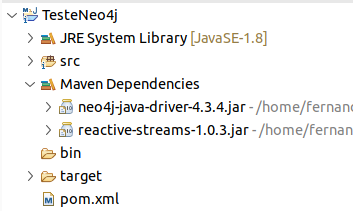
\includegraphics[width=0.4\textwidth]{imagens/dependenciasMaven}
  \caption{Dependências do Maven}
\end{figure}

Observamos que na pasta \textbf{Maven Dependencias} foi baixado a versão 2.8.1 do driver Jedis - Isso não é erro de digitação realmente o driver se escreve com "J".

\subsection{Exemplo Prático}
Estamos prontos para testarmos a conexão entre Redis e Java. Criamos um pequeno exemplo que nos auxiliará como teste, uma classe chamada \textbf{Hello} no pacote \textbf{decus.com} e inserimos nesta a seguinte codificação:
\begin{lstlisting}[]
package decus.com;

import static org.neo4j.driver.Values.parameters;

import org.neo4j.driver.AuthTokens;
import org.neo4j.driver.Driver;
import org.neo4j.driver.GraphDatabase;
import org.neo4j.driver.Result;
import org.neo4j.driver.Session;
import org.neo4j.driver.Transaction;
import org.neo4j.driver.TransactionWork;

public class Exemplo implements AutoCloseable {
  private final Driver driver;
  
  public Exemplo(String uri, String user, String password) {
    driver = GraphDatabase.driver(uri, AuthTokens.basic(user, password));
  }
  
  @Override
  public void close() throws Exception {
    driver.close();
  }
  
  public void exemplo() {
    try (Session session = driver.session()) {
      String saudacao = session.writeTransaction(new TransactionWork<String>() {
      @Override
      public String execute(Transaction tx) {
        Result result = tx.run(
          "CREATE (s:Saudacao) SET s.mensagem = $mensagem " + 
          "RETURN s.mensagem + ', from node ' + id(s)",
          parameters("mensagem", "Hello World!"));
          return result.single().get(0).asString();
        }
      });
      System.out.println(saudacao);
    }
  }

  public static void main(String... args) throws Exception {
    try (Exemplo hello = new Exemplo("bolt://localhost:7687", "neo4j", "test")) {
      hello.exemplo();
    }
  }
}
\end{lstlisting}

Penso que usar o Neo4j para escrever "Hello World!" seja demais, porém pensemos nisso como exemplo para entendermos como tudo funciona, no construtor da classe passamos os parâmetros para nos conectamos ao driver, por implementação da \textit{AutoCloseable} sobrepomos o método \textit{close()} que será responsável por encerra a conexão. Começando nossa execução pelo método \textit{main()} criamos um objeto da classe no qual definimos a URI (caminho de conexão), usuário e senha (que criamos para nosso contêiner) e chamamos o método \textit{exemplo()}). Esse inicia uma sessão que implementa um do tipo \textit{TransactionWork}, exige uma implementação do método \textit{execute(Transaction)} e nesse passamos o comando Cypher que desejamos enviar para o Neo4j.

Foi como usar um canhão para matar um mosquito, porém estrutura básica é esta e a partir dela faremos as modificações para compreendermos como funciona a comunicação. Vamos mudar o método \textit{exemplo()} para a seguinte codificação:
\begin{lstlisting}[]
  public void exemplo() {
    try (Session session = driver.session()) {
      session.run("CREATE (:Pessoa {nome: $nome, modelo_carteira : $modelo})", 
        parameters("nome", "Fernando", "modelo", "AB") 
      );
      session.run("CREATE (:Pessoa {nome: $nome, modelo_carteira : $modelo})", 
        parameters("nome", "Anselmo", "modelo", "A") 
      );
      session.run("CREATE (:Automovel {nome: $nome})", 
        parameters("nome", "Ecosport") 
      );
    }
  }
\end{lstlisting}

Assim teremos nossos dados criados sem muitas modificações conforme vimos na seção \textbf{Cypher}. Para criarmos os relacionamentos vamos fazer um pouco diferente (novamente substituindo o método \textit{exemplo()}):

\begin{lstlisting}[]
  public void exemplo() {
    final String nomeAutomovel = "Ecosport";
    final String [] nomes = {"Fernando", "Anselmo"};
    for (String nomePessoa: nomes) {
      try (Session session = driver.session()) {
        session.run("MATCH (p:Pessoa { nome: $nomePessoa }) "
          + "OPTIONAL MATCH (a:Automovel { nome: $nomeAutomovel }) "
          + "CREATE (p)-[:DONA]->(a)", 
          parameters("nomePessoa", nomePessoa, "nomeAutomovel", nomeAutomovel) 
        );
      }
    }
  }
\end{lstlisting}

E podemos trazer os dados com (novamente substitua o método \textit{exemplo()}):

\begin{lstlisting}[]
  private Result showBase(final Transaction tx) {
    Result result = tx.run("MATCH (a)-[:DONA]->(b) RETURN a.nome, b.nome");
    while (result.hasNext()) {
      Record r = result.next();
      System.out
        .println(String.format("%s proprietário de %s", r.get("a.nome").asString(), r.get("b.nome").toString()));
    }
    return result;
  }

  private void exemplo() {
    try (Session session = driver.session()) {
      session.writeTransaction(tx -> showBase(tx));
    }
  }
\end{lstlisting}

No método \textit{exemplo()} criamos a seção que através de uma transação executará o método \textit{showBase()}, nesse temos a execução de um comando \textbf{MATCH} que retorna os relacionamentos encontrados, basicamente este objeto da classe \textbf{Result} pode ser comparado com um MAPA, basta percorrê-lo e obter os resultados com um \textbf{get}.

Resumidamente, tudo que vimos na seção \textbf{Cypher} podemos aplicar com a linguagem Java, porém antes de encerrarmos esta parte vamos criar uma nova classe e fazer um programa que com toda certeza seria um modelo completo ideal para iniciarmos nossas explorações.

\subsection{Locadora Java}
Neste exemplo um pouco mais completo temos um interessante ponto de partida para a construção do que pode ser um sistema sobre Aluguel de Veículos que pode abranger relacionamentos entre vendedores, clientes e empresas.
\begin{lstlisting}[]
package decus.com;

import static org.neo4j.driver.SessionConfig.builder;
import static org.neo4j.driver.Values.parameters;
import java.util.ArrayList;
import java.util.List;
import org.neo4j.driver.AccessMode;
import org.neo4j.driver.AuthTokens;
import org.neo4j.driver.Bookmark;
import org.neo4j.driver.Driver;
import org.neo4j.driver.GraphDatabase;
import org.neo4j.driver.Record;
import org.neo4j.driver.Result;
import org.neo4j.driver.Session;
import org.neo4j.driver.Transaction;

public class Locadora implements AutoCloseable {

  private final Driver driver;
  
  public Locadora(String uri, String user, String password) {
    driver = GraphDatabase.driver(uri, AuthTokens.basic(user, password));
  }

  @Override
  public void close() throws Exception {
    driver.close();
  }

  private Result addEmpresa(final Transaction tx, final String nome) {
    return tx.run("CREATE (:Empresa {nome: $nome})", parameters("nome", nome));
  }

  private Result addPessoa(final Transaction tx, final String nome) {
    return tx.run("CREATE (:Pessoa {nome: $nome})", parameters("nome", nome));
  }

  private Result empregado(final Transaction tx, final String pessoa, final String empresa) {
    return tx.run("MATCH (p:Pessoa {nome: $pessoa_nome}) " +
    "MATCH (e:Empresa {nome: $empresa_nome}) " +
    "CREATE (p)-[:TRABALHA_PARA]->(e)",
    parameters("pessoa_nome", pessoa, "empresa_nome", empresa));
  }

  private Result fazerAmigos(final Transaction tx, final String pessoa1, final String pessoa2) {
    return tx.run(
    "MATCH (a:Pessoa {nome: $pessoa_1}) " +
    "MATCH (b:Pessoa {nome: $pessoa_2}) " +
    "MERGE (a)-[:CONHECE]->(b)",
    parameters("pessoa_1", pessoa1, "pessoa_2", pessoa2));
  }

  private Result mostrarAmizade(final Transaction tx) {
    Result result = tx.run("MATCH (a)-[:CONHECE]->(b) RETURN a.nome, b.nome");
    while (result.hasNext()) {
      Record r = result.next();
      System.out.println(String.format("%s conhece %s",
      r.get("a.nome").asString(),
      r.get("b.nome").toString()));
    }
    return result;
  }

  public void construir() {
    List<Bookmark> savedBookmarks = new ArrayList<>();
    try (Session s1 = driver.session(
        builder()
          .withDefaultAccessMode(AccessMode.WRITE).build())) {
      s1.writeTransaction(tx -> addEmpresa(tx, "Bros Carros"));
      s1.writeTransaction(tx -> addPessoa(tx, "Mario"));
      s1.writeTransaction(tx -> empregado(tx, "Mario", "Bros Carros"));
      savedBookmarks.add(s1.lastBookmark());
    }
    try (Session s2 = driver.session(
        builder()
          .withDefaultAccessMode(AccessMode.WRITE).build())) {
      s2.writeTransaction(tx -> addEmpresa(tx, "Usina Carros"));
      s2.writeTransaction(tx -> addPessoa(tx, "Luigi"));
      s2.writeTransaction(tx -> empregado(tx, "Luigi", "Usina Carros"));
      savedBookmarks.add(s2.lastBookmark());
    }
    try (Session s3 = driver.session(
      builder()
        .withDefaultAccessMode(AccessMode.WRITE)
        .withBookmarks(savedBookmarks).build())) {
      s3.writeTransaction(tx -> fazerAmigos(tx, "Mario", "Luigi"));
      s3.readTransaction(this::mostrarAmizade);
    }
  }

  public static void main(String... args) throws Exception {
    try (Locadora loc = new Locadora("bolt://localhost:7687", "neo4j", "test")) {
      loc.construir();
    }
  }
}
\end{lstlisting}

E ao término da execução dessa classe o seguinte relacionamento será montado:
\begin{figure}[H]
	\centering
	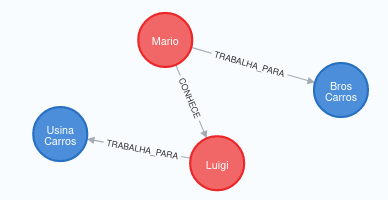
\includegraphics[width=0.4\textwidth]{imagens/locadora}
	\caption{Relacionamentos da Locadora}
\end{figure}

Observaremos cada seção no método \textbf{construir()} é formado por um conjunto lógico de chamadas, com uma execução em formato de \textit{Pipeline} para cada transação a ser chamada dentro de uma seção. Creio que essa ser a forma mais elegante de se construir em Java.